\section{“你吃了吗?”}
基本在所有国家,一般两人见面,两人见面,都要问 :“你也好呢吧。回答:“好呢。”两人的对话就像写新闻消息的导语,接下来才谈正事。在德国也是如此,而在中国往往见面,特别是熟人见面时,所说的第一句话却是“你吃了吗?”。对中国来说这是一句非常真诚的问候,而不是限于礼节的客套。

\begin{figure}
    \centering
    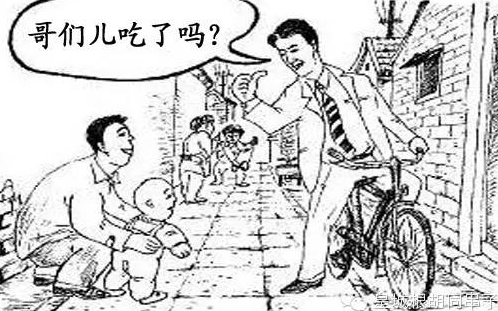
\includegraphics[width=0.6\linewidth]{hast_du_gegessen}
    \caption{中国人见面常见的问候方式}
\end{figure}
在中国人看来,如果见面问候给人造成了心理压力,那对方回不回答彼此都很尴尬,所以,才有了约定俗成的这句“你吃了吗?”以其经典的特色延续了下来。大众广庭众目睽睽之下这样热情地一问,既体现了自己待人的热情,又不至于让对方难堪,也拉近了和对方的关系。

这一句问候的体现了中国饮食对中国人的重要性。所谓民以食为天,对于中国人来说吃是一等一的大事,尤其是在物资短缺的年代。饮食文化在与中国人民的交际中占有举足重轻的地位,主人宴请往往会给客人敬酒,夹菜,以示地主之谊。在中国,饮食已上升到了一种几乎超越其他一切物质形态和精神形态的举足轻重的东西。

中国传统的烹调方法,会因各大菜系的有所不同;同一菜点的口味不同风味与特点而主辅料的搭配,也会因为厨师的专长和喜好而有所不同,甚至还会因为厨师临场情绪的变化,做出某种即兴的发挥。这也体现中国文化,顺应自然,重视经验,轻视创新实验。

而在德国, 饮食仅仅作为一种生存的必要手段和交际方式。 林语堂先生曾说。 西方人的饮食观念不同于中国,英美人仅以“吃” 为对一个生物的机器注入燃料,保证其正常的运行,只要 他们吃了以后能保持身体健康、 结实,足以抵御病菌、 疾病的攻击,其他皆在不足道中。 不难看出,吃虽然重要,但是从文化的意义上看,在西方国家只是停留在简单的交流、 交际的层面上,并没有像在中国那样被赋予更多、更为重要的使命。

\subsection{ 主题拓展}
不仅仅是问候语,中国人的日常用语也有和饮食相关的表达:
\begin{enumerate}
\item 
职业 - 饭碗
\item
 幸福 - 陶醉
\item
 嫉妒 - 吃醋
\end{enumerate}